\chapter{Results}
\label{Results}
We have a lot of ways to check if solutions for both problems are working correctly. The testing for forward kinematics is trivial; we just move the end effector to a position and we just check if forward kinematics returned the correct position and orientation. On the other hand, the testing of inverse kinematics was more difficult because we must give a valid target point if we want inverse kinematics to return a solution.\\
The problem is that we don't know the work space for the end effectors of NAO. So, we came up with another way to validate our solution. We moved one end effector to a random position, then we took the position and the orientation of this point from forward kinematics and then we assigned this point as the target point for inverse kinematics. Then we checked if inverse kinematics found a solution and we know that the solution inverse kinematics returned is correct, because there is a step of forward kinematics inside inverse kinematics that validates the output.\\
In table~\ref{times} we can see the execution times for each function (of inverse kinematics) in microseconds (us). Unfortunately, we can't compare these times with the Aldebaran's solution execution time, because it is not independent and along with the solution for inverse kinematics, it does the movement of the joints of the chain. So, we can't extract ``clean'' times from the execution.\\
We made two demos to present kinematics in real world. The first demo tests inverse kinematics of the arm along with forward kinematics of the legs. The second demo is more complicated and checks inverse kinematics of the legs and the calculation of the center of mass.\\
\begin{table}[!h]
\centering
\caption{Execution Times}
\vspace*{0.06cm}
\begin{tabular}{|c|c|}
\hline
\textbf{Function} & \textbf{Time (us)}\\ \hline
left leg & 10 \\
\hline
\end{tabular}
\label{times}
\end{table}
\section{Demo Program}
\textbf{Point To The Ball}\\
In the first demo we want to make NAO point to the ball with the hands. We used, along with the kinematics, the vision~\cite{orfanoudakis2011} and the world state model of the robot. First, NAO searches for the ball and when it finds it, NAO points to the ball with one or two hands. With the help of the world state model, if NAO loses the ball, it can continue to point to the area that the ball must be according to the last vision observations.\\
The ball observation can be described as a \(two\)-dimensional point without orientation. The coordination of the ball is described as polar coordinates, so we have the distance and the angle of the observation relatively to the projection of the torso on the floor. We must now move this point from \(two\)-dimensions to \(three\)-dimensions and give it an orientation. First, we transform the polar coordinates to Cartesian coordinates ($ p_x,p_y $) and we add the height of the torso as the \(p_z\). Now we know the position in the \(three\)-dimensional space and we also know that \(a_x\) equals to zero because we are only rotating \(y\)-axis (up/down) and \(z\)-axis (right/left). To find the two other angles, we get the straight line that connects the point of the ball and the position of the shoulder pitch joint relatively to the torso frame. Then we have that \(a_y\) equals to the angle between this line and the \(y\)-axis and similarly we find the \(a_z\). Now we must calculate the position of the target point, which is in the line and from a distance \(d\) from the joint, where \(d\) is the size of the stretched arm (this is the maximum size of the arm). We need to bring the target point to that distance, because only then it will be a valid target point for inverse kinematics. We do this operation two times, one for each arm (different position of the shoulder joint) and then we give to inverse kinematics for left and right arm the resulted target points. Below there are images from the demo:
\begin{figure}[!h]
\centerline{
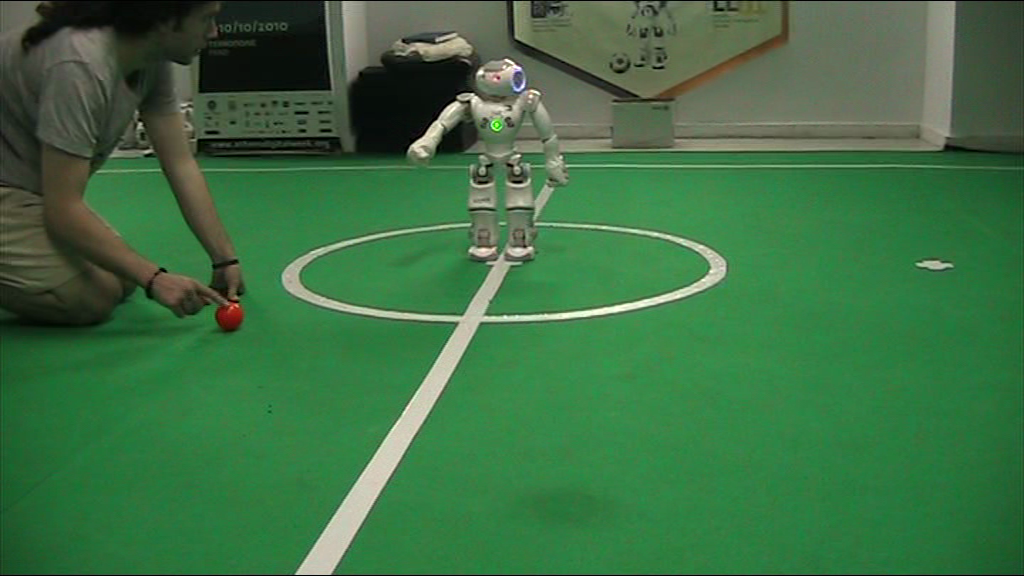
\includegraphics[width=0.32\textwidth]{Figures/Demo1/1.png}
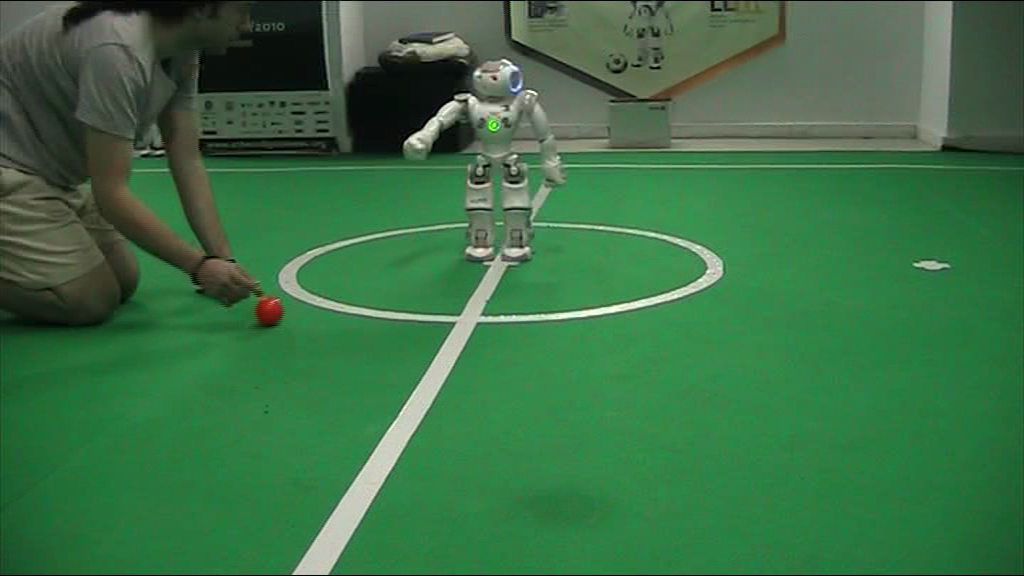
\includegraphics[width=0.32\textwidth]{Figures/Demo1/2.png}
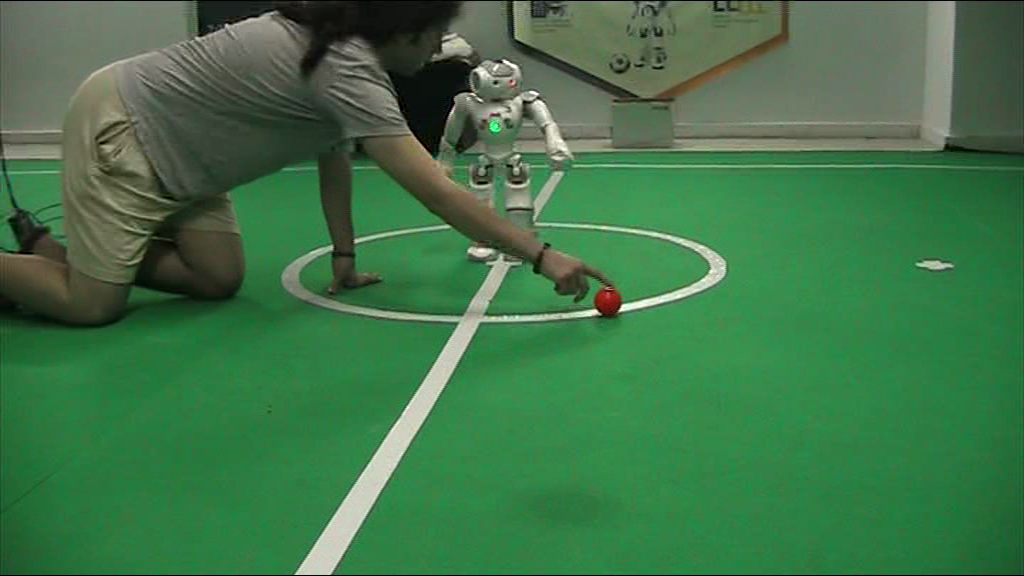
\includegraphics[width=0.32\textwidth]{Figures/Demo1/3.png}
}
\vspace*{0.06cm}
\centerline{
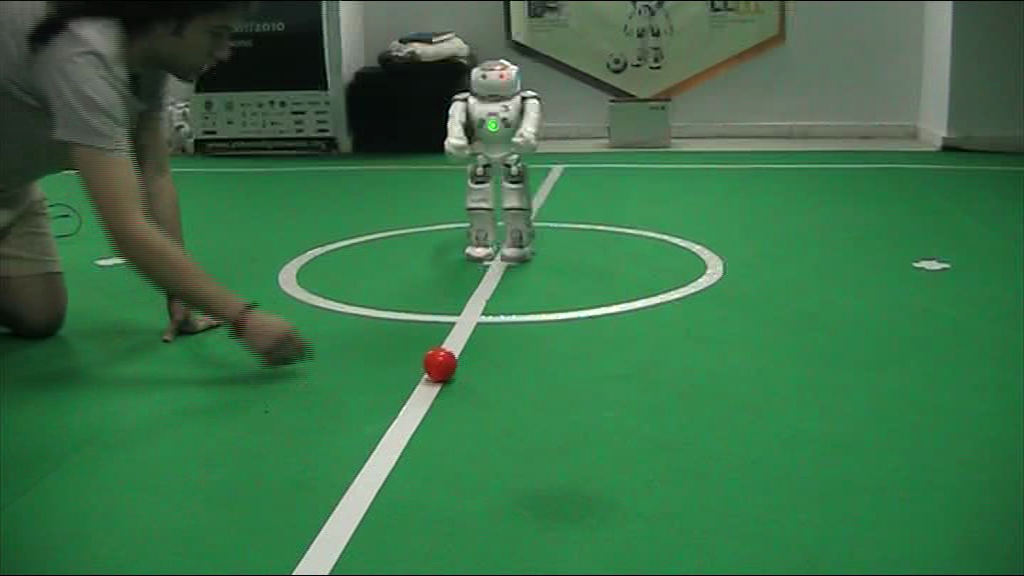
\includegraphics[width=0.32\textwidth]{Figures/Demo1/4.png}
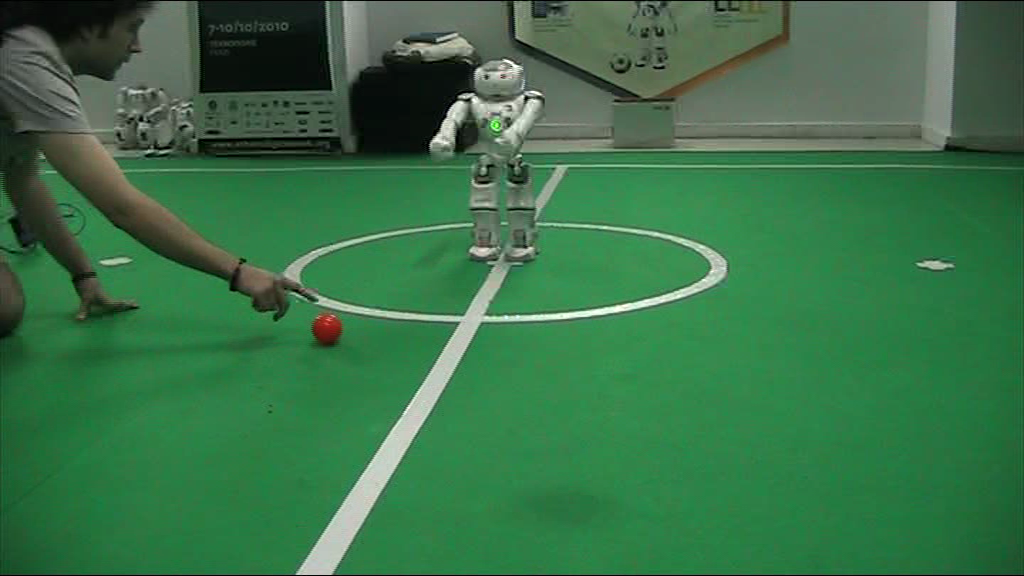
\includegraphics[width=0.32\textwidth]{Figures/Demo1/5.png}
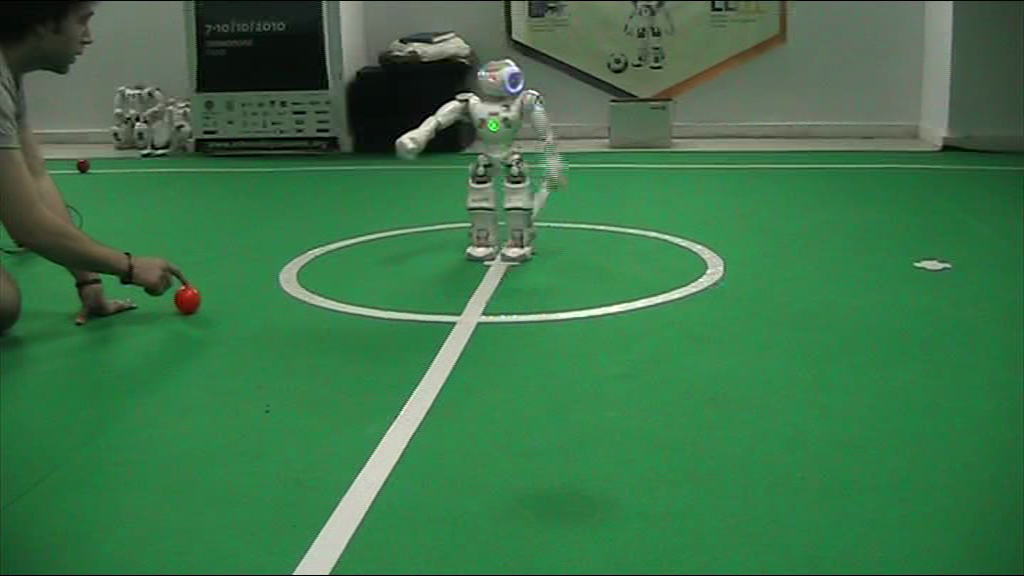
\includegraphics[width=0.32\textwidth]{Figures/Demo1/6.png}
}
\vspace{-0.1cm}
\caption{Point the ball using forward and inverse kinematics}
\label{demo1}
\vspace*{0.5cm}
\end{figure}\\
\textbf{Balancing Using The Center Of Mass}\\
In the second demo we want to make NAO to move one of its legs to the point of the projection of the CoM on the floor, so, we will have a very basic balancing system. First of all, we must calculate the position of the CoM using forward kinematics. Now we have the CoM position relatively to the torso frame. The problem is that the torso frame is never parallel to the floor. Thus, we get from the gyro-meters the angleX and angleY of the torso plain. Now we can take the position of the CoM relatively to the rotated torso:
\[
	T_{\text{rotated}} = R_y(\text{angleY})R_x(\text{angleX})A_{\text{CoM}}
\]
Then we put a custom value to \(p_z\) which represents the desired torso height from the floor, so, now we have \(T_{\text{rotated}'}\). Now we must rotate back to the torso frame, so:
\[
	T_{\text{final}} = \left(R_y(\text{angleY})R_x(\text{angleX})\right)^{-1}T_{\text{rotated}'}
\]
Finally, we set  \(p_x\), \(p_y\) and \(p_z\) from \(T_{\text{final}}\) as the target point for inverse kinematics and we set \(a_x = -\)anglex, \(a_y = -\)angleY and \(a_z = 0\) as the target rotation, because we don't care about rotation around \(z\)-axis. Now the target point is the projection of the CoM to the floor and the rotation of the end effector is parallel to the frame of the floor.\\
In the figures below we can see that the foot is always parallel to the floor. It happens some times, that some robots have displaced inertial unit (accelerometers and gyro-meters). On these robots we can see that the foot is not parallel to the floor but this is a hardware problem and not a kinematics problem.
\begin{figure}[!h]
\centerline{
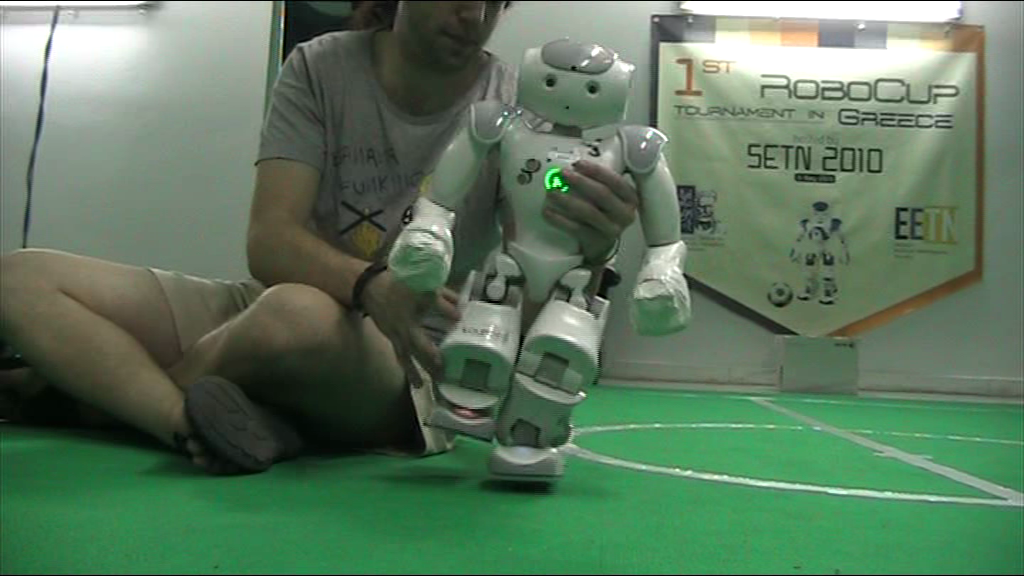
\includegraphics[width=0.32\textwidth]{Figures/Demo2/1.png}
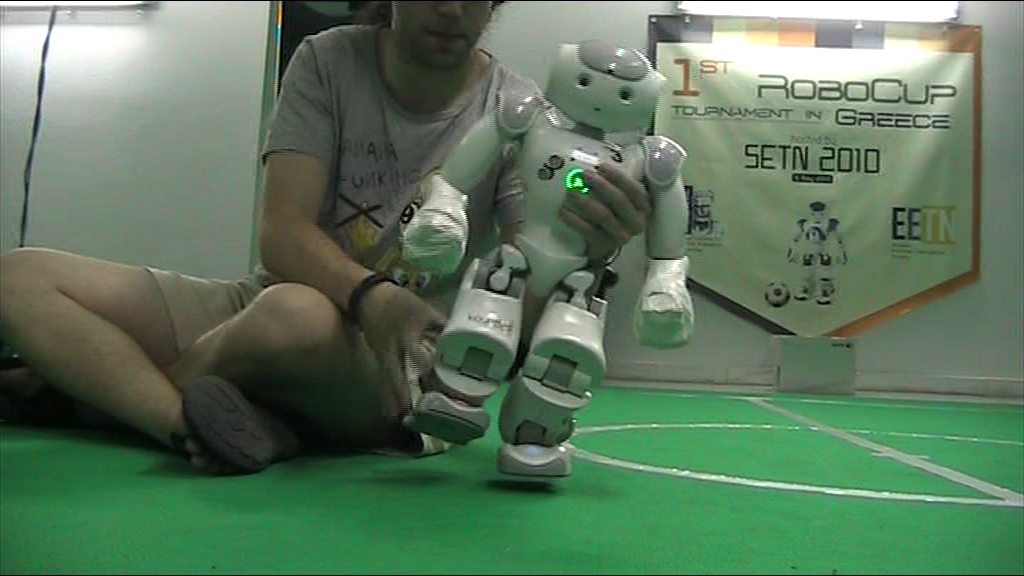
\includegraphics[width=0.32\textwidth]{Figures/Demo2/2.png}
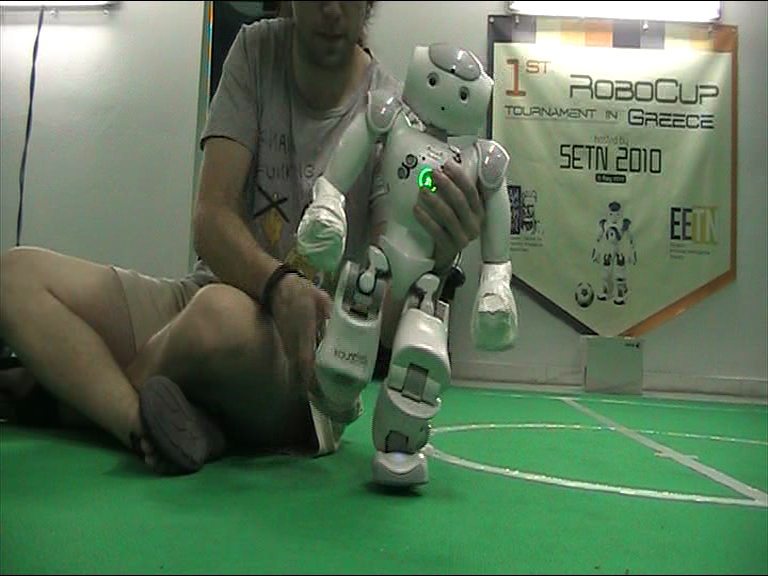
\includegraphics[width=0.32\textwidth]{Figures/Demo2/3.png}
}
\vspace*{0.06cm}
\centerline{
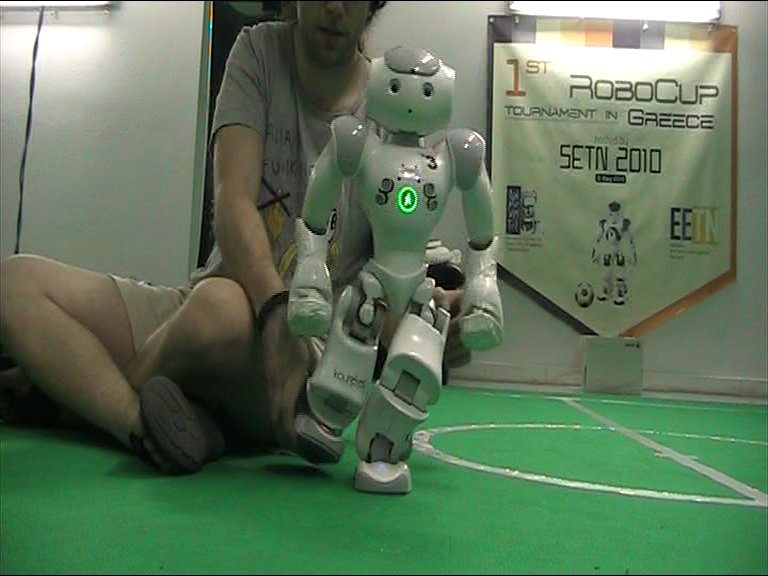
\includegraphics[width=0.32\textwidth]{Figures/Demo2/4.png}
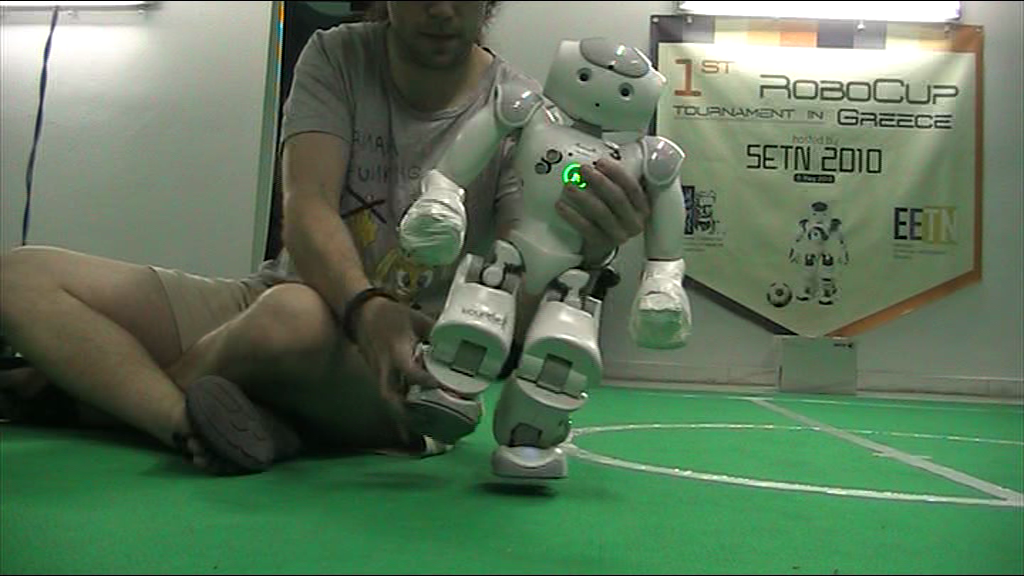
\includegraphics[width=0.32\textwidth]{Figures/Demo2/5.png}
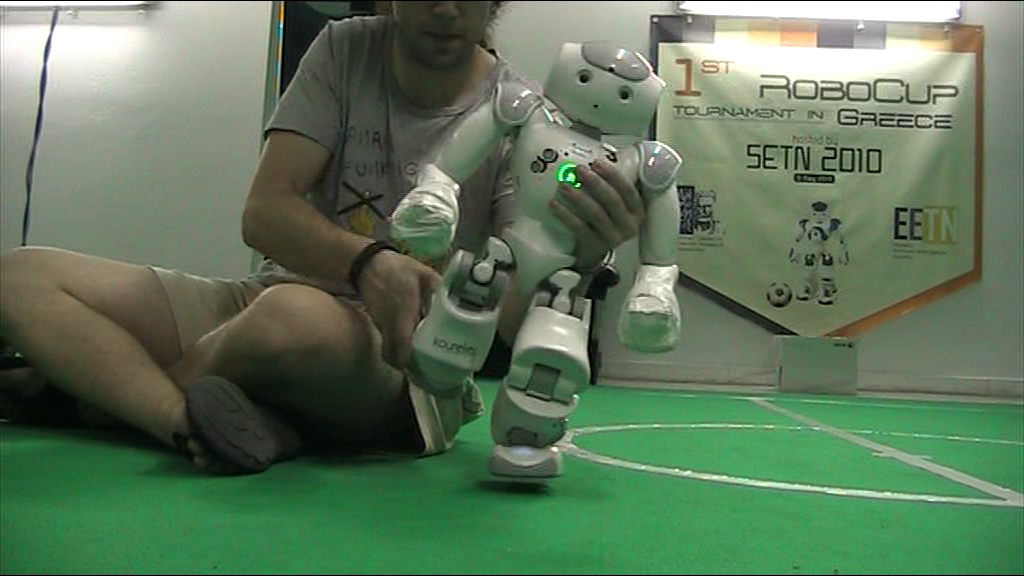
\includegraphics[width=0.32\textwidth]{Figures/Demo2/6.png}
}
\vspace{-0.1cm}
\caption{Basic balance system using center of mass}
\label{demo1}
\vspace*{0.5cm}
\end{figure}
% ------------------------------------------------------------------------

%%% Local Variables:
%%% mode: latex
%%% TeX-master: "../thesis"
%%% End: